\Chapter{Megvalósítás}

Ebben a fejezetben kerül részletes bemutatásra a program implementációjának folyamata, kiegészítve a nehézségekkel, problémákkal és azok megoldásával.

\section{Kezdeti Megoldások}

Kezdetben a program megvalósítása egy nagyon egyszerű
\begin{itemize}
	\item \texttt{index.html}
	\item \texttt{index.css}
	\item \texttt{index.js}
\end{itemize}
fájl trióval történt.\\

Nagy méretű projekt esetében ez a megoldás nem célravezető, azonban ez a felépítés az elején pont megfelelő arra, hogy a tervezett feladatok megvalósításához szükséges funkciók, adatok felkutatásához és implementálásához adjon egy "homokozót".

Eleinte a program megvalósítása szorosan együtt járt az \textbf{npm} technológia vizsgálatával, mivel a szükséges adatok megszerzése az npm-hez kötődik.

A megoldandó problémák az alábbiak:

\begin{itemize}
	\item A csomag függőségi és egyéb adatainak megszerzése, tárolása
	\item A megszerzett adatokat valamilyen eszközzel ábrázolni, lehetőleg valamilyen npm csomaggal
	\item A programot npm csomaggá strukturálni, amely front-end alkalmazásként működik majd
\end{itemize}


\subsection{Felhasználói Felület}

A szoftver megvalósításának első lépése a UI kivitelezése volt. A felhasználói felülethez csak a HTML és CSS fájlok kellettek, illetve a tervezett módon a már kész felhasználói felület köré szerveződik a program, így tökéletes első lépésnek.

Habár az alap elrendezést és megjelenést most kapja meg, a későbbiekben még szükséges lesz átalakításra, hogy statikus oldal helyett egy single-page applikációként viselkedjen, de az majd csak JavaScript segítségével kerül megvalósításra.

A UI látványtervből kiindulva, felosztottam a weboldalt 25\% és 75\% arányban a "vászon" javára. A vásznon fog történni minden nagy területet igénylő ábra megjelenítése. Az oldalsó menü a tervek szerint két különböző tartalmat fog megjeleníteni a felhasználási módnak megfelelően.

Korábban szó esett arról, hogy a weboldal világos és sötét módban is elérhető lesz. Ennek a megvalósítása szintén JavaScript használatát vonzza maga után, így elsőként alapértelmezett sötét módban készül a UI.

\subsection{Csomagok Vizsgálata}

A szoftver lényegi része a csomagok vizsgálatához kötődik. Az npm csomagok esetében minden csomag rendelkezik egy \texttt{package.json} fájllal. Ebben a fájlban az aktuális csomagról létező fontosabb információk nagy része megtalálható. Ennek a vizsgálatával kinyerhetők az aktuális csomag függőségei. A módszerrel azonban több \textbf{probléma} is van:

\begin{itemize}
	\item Csak a rendszerre telepített csomagok \texttt{package.json} fájlja érhető el
	\item Az aktuális csomagról csak a direkt függőségeket tárolja, így rekurzív keresést fog eredményezni
	\item A rendszernek rendelkeznie kéne a teljes npm csomag adatbázissal, hogy bármely csomag esetében működjön, ami nagyon nagy tárigényű lenne
	\item Bár a NodeJS ad lehetőséget a fájlrendszer kezelésére, alapvetően a JavaScriptet nem erre találták ki.
\end{itemize} 

\noindent \textbf{Megoldás:}\\

A kutatás során több hasonló témájú programot is megnéztem. Ezek közül a legérdekesebbnek a már említett \textbf{npmgraph.an} bizonyult. Mivel interaktív, webes programként működött, így kíváncsivá tett. 

Megfigyeltem, hogy HTTP kéréseket intéz egy hivatkozás felé és így találtam rá az \textbf{npm Registry}-re. Gyakorlatilag minden szükséges adatot tartalmaz az npm csomagadatbázisban található csomagokról, verziókra lebontva, így az adatok megszerzéséről szóló igényeket teljes mértékben kielégíti.

Így az alábbi nem túl elegáns, a későbbiekben megváltoztatandó, azonban működő konstrukcióval sikeresen implementáltam egy csomag adatainak a lekérését:

\begin{cpp}
function getPackage(packageName, packageVersion=""){
	let pkgData = packageName+"/"+packageVersion;
	let registryUrl = "https://registry.npmjs.cf/"+pkgData;
	let xmlHttp = new XMLHttpRequest();
	xmlHttp.open( "GET", registryUrl, false );
	xmlHttp.send( null );
	return JSON.parse(xmlHttp.responseText)
}
\end{cpp}

A megoldás ebben a formában nem foglalkozik se hibakezeléssel, se azzal, hogy szinkron jellege miatt a weboldal működését blokkolja egészen addig, míg a kérés nem teljesült, azonban az adatok megszerzése a cél, hogy megvizsgáljam azok milyen formában érkeznek, hogy írni tudjak feldolgozó funkciókat.

\section{Tényleges Implementáció} 

A \hyperlink{section.4.1}{kezdeti megoldások} szakaszban elért eredményekkel a projekt abba a szakaszba lépett, ahol megtörténhet a tényleges implementálásról. Mivel a csomagadatok lekérdezésének problémája megoldódott, így gond nélkül lehet rekurzív keresést implementálni, amelynek eredményeként megkaphatjuk egy adott csomag adott verziójának összes függőségét.

Ebben a szakaszban részletesen be fogom mutatni a program különböző részeinek felépítését és működését, illetve az npm funkciókat, amikre szükség van a feladatok elvégzésében.

\subsection{Csomag Szerkezet}
Az npm csomagok szerkezetére vannak megkötések, így a projekt szerkezetét is ilyen formára kell hozni. Elkészült hozzá a \texttt{package.json} fájl, amely tartalmaz minden kötelező és releváns opcionális mezőt. A csomag a \textbf{package-examiner} fantázianevet kapta.   

A csomag belépési pontja, a \texttt{package.json}-ban is jelzett \texttt{main.js}. A csomag funkcionális szerkezete az alábbi módon néz ki:

\begin{cpp}
./	
	src
		- scripts
		- styles
		- templates
		- app.js
		- main.js
	public
		- index.html
	package.json
	package-lock.json
	README.md	
\end{cpp}

Mint látható csak az \texttt{index} HTML fájl létezik, ennek oka a következő szakaszban részletezésre kerül.

\subsection{Single-Page UI}

A Single Page Application, azaz SPA lényege, hogy egy oldalra dinamikusan tölti be a tartalmat, nem történik új lap nyitása, se újratöltés.

Ennek a megvalósítására több technológia létezik, többek között a jQuery könyvtár is. A program úgynevezett "JavaScript Template"-ekkel való megoldást alkalmazza, amely során JavaScript fájlokban hoz létre HTML sablonokat és azokat exportálja, majd az applikáció felhasználási módtól függően dinamikusan tölti be azokat.

\pagebreak

\textbf{Egy ilyen exportálható JavaScript Template szintaktikája:}

\begin{cpp}
	const Template = () => {
		const template = `
		#Some HTML code
		`;
		return template;
	};

	export default Template;
\end{cpp}

A program az alábbi sablonokat tartalmazza:
\begin{cpp}
./templates/	
	Sidebar
	- Examiner.js
	- Statistics.js
	Canvas.js
	Sidebar.js
\end{cpp}

Az Sidebar és Canvas sablonokat az app.js fájl tölti be automatikusan az index.html-be, ezek konstansan részét képezik az index tartalmának. A Sidebar és a Canvas tartalmának egy része azonban felhasználási módtól függően változik. 

Az Examiner-t egy csomag, a Statistics-t több csomag vizsgálata estén tölti be.

A két funkcionalitási mód közötti váltást egy "Switch Mode" gomb teszi lehetővé.

\begin{figure}[!h]
	\centering
	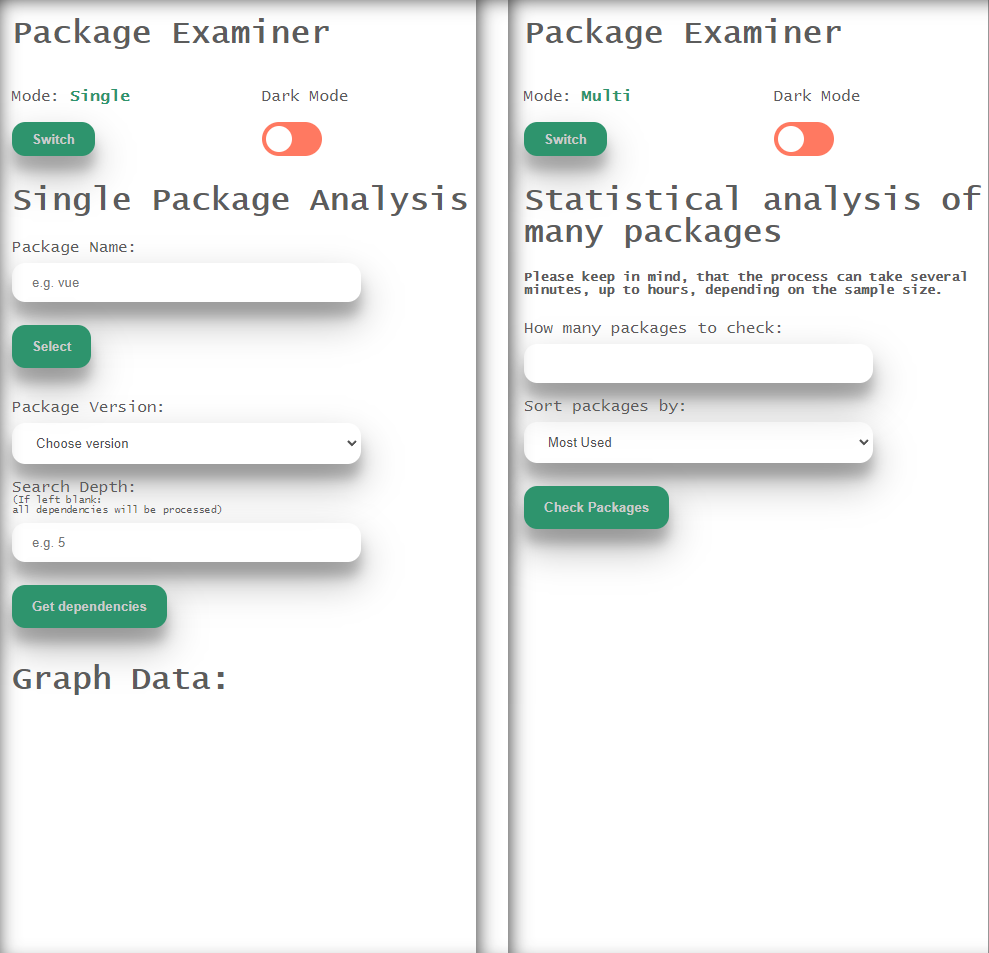
\includegraphics[scale=0.3]{images/ui_modes.png}
	\caption{Single / Multi Package Sidebar}
	\label{fig:ui_modes}
\end{figure}

Amennyiben a Registry-ben csak a csomagnévre keresünk rá, akkor nem fogunk függőségeket visszakapni, mivel itt általános információk vannak a csomagról, nem pedig működési információk. Konkrét információt a verzió megadásával tudunk megszerezni.

Az \textbf{Single Package Analysis} esetén, ha létező csomagra keresünk rá, akkor automatikusan felölti a Package Version listát. Mivel a Registry-ben szükséges verziók szerint keresni, ez biztosítja a keresés sikerességét.


\pagebreak

A Sidebar továbbá tartalmaz egy konstansan jelen lévő kapcsolót, amellyel a világos és sötét megjelenítési mód között lehet választani, az alapértelmezett mód a sötét, viszont \underline{nyomtatási szempontból} a \textbf{világos módot} fogom használni az ábrákhoz. 

\begin{figure}[!h]
	\centering
	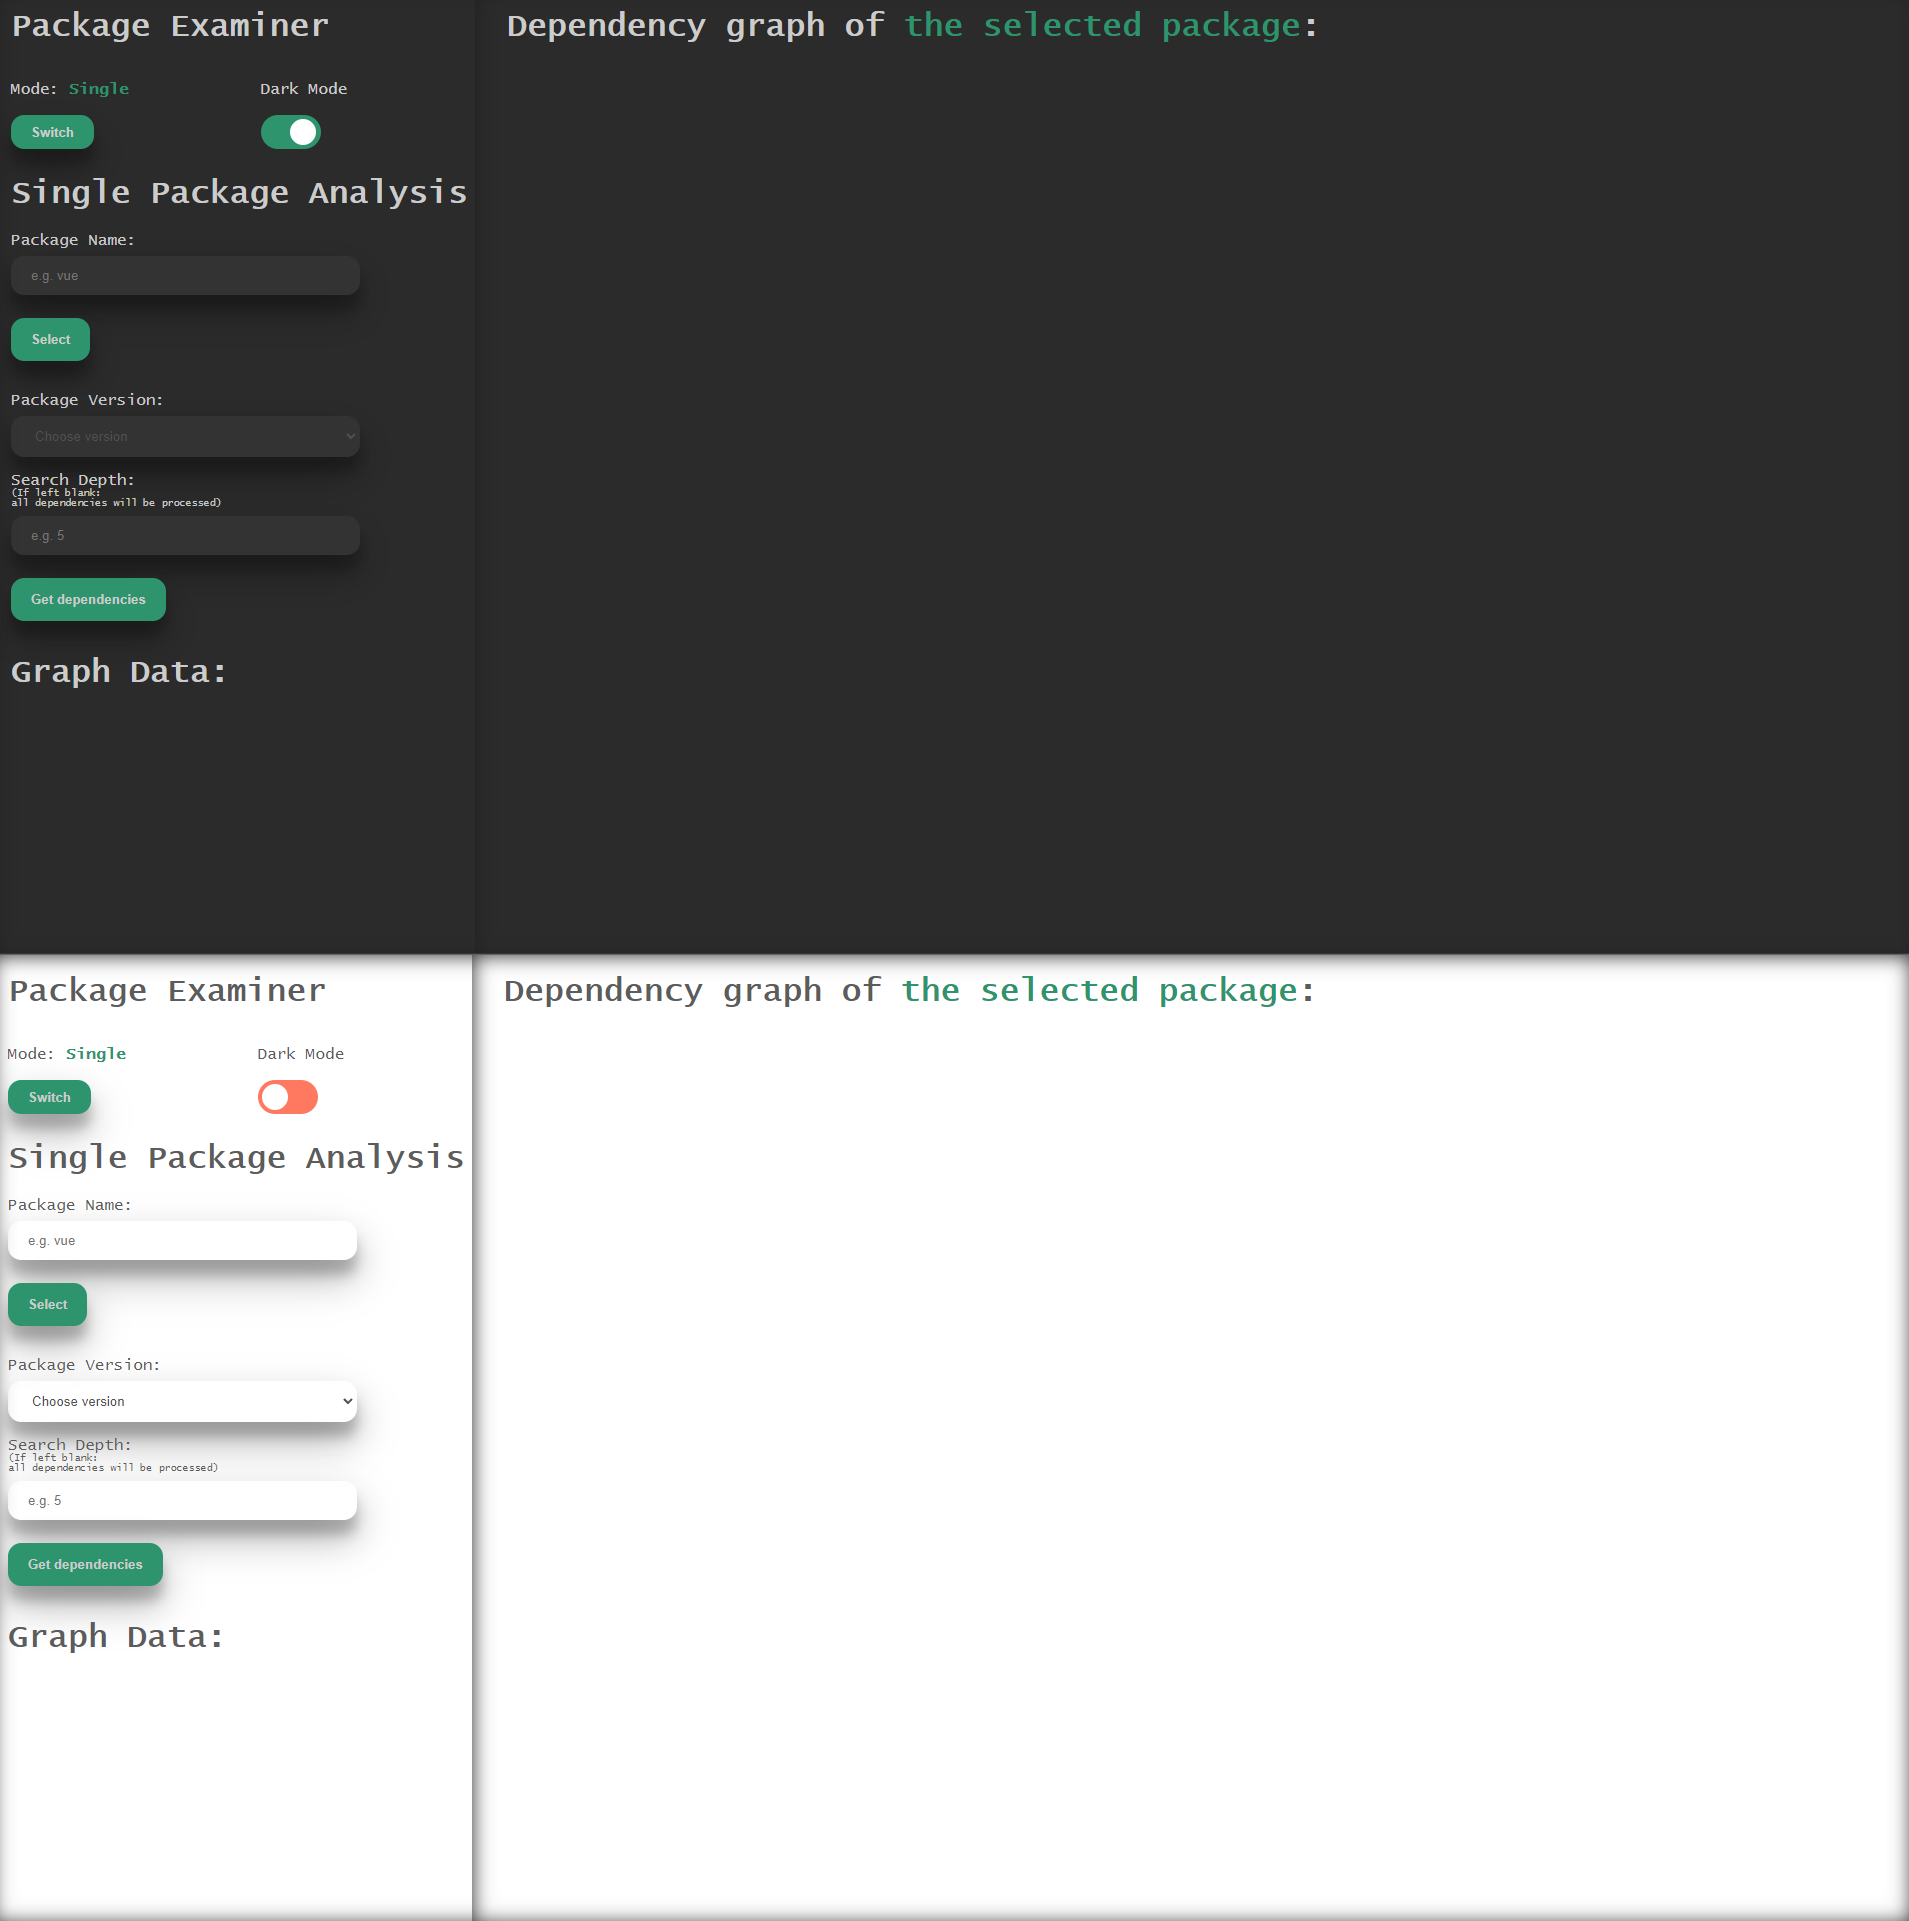
\includegraphics[scale=0.1]{images/ui_darkmode.png}
	\caption{UI Sötét/Világos mód}
	\label{fig:ui_darkmode}
\end{figure}

A csomagok adatainak lekérdezését, függőségek összegyűjtését, elemzését és ábrázolását végző funkciókat a következő "lekezelő" funkció indítja el, amint a szükséges információk ki vannak gyűjtve:

\begin{cpp}
window.handleFormEvents = (event) => {
	event.preventDefault();
	submitForm(event.target.id);
};
\end{cpp}

\subsection{Adatgyűjtés}

Az adatok lekérésére két különböző modul áll rendelkezésre, a \textbf{getPackage.js} és a \textbf{searchPackages.js}

A program HTML formok küldés eseményére reagál, majd ezeket lekezeli és a form típusától függően hív meg függvényeket. Ezt a \textbf{handleSideBarEvents.js} modul fogja végezni, mely az alábbiak szerint dönti el, hogy mely funkciókat hívja meg:

\begin{cpp}
function submitForm(form){
	switch (form) {
		case "packageForm":
		getPackageData();
		break;
		case "graphingForm":
		makeGraph();
		break;
		case "statForm":
		makeStat();
		break;
		default:
		break;
	}
}
\end{cpp}

\noindent\textbf{getPackageData()}
\begin{itemize}
	\item Ez a funkció felelős a "Package Version" Select DOM elem listájának feltöltéséért. 
	\item Amennyiben nem található a csomag, hibát fog dobni
	\item Közvetlenül támaszkodik a \textbf{getPackage.js} modulra
\end{itemize}

\noindent\textbf{makeGraph()}
\begin{itemize}
	\item Ez a funkció felelős a kiválasztott csomag függőségei gráfjának megalkotásáért, megrajzolásáért, majd pedig elemzéséért
	\item Amennyiben nincs kiválasztva a verzió, hibát fog dobni.
	\item Közvetetten támaszkodik a \textbf{getPackage.js} modulra
\end{itemize}

\noindent\textbf{getPackageData()}
\begin{itemize}
	\item Ez a funkció felelős több csomagos mód esetén a megadott paraméterek szerinti csomagok összegyűjtéséért, függőségi elemzéséért és statisztikai ábrázolásáért.
	\item Amennyiben nem található a csomag, hibát fog dobni
	\item Közvetletetten támaszkodik a \textbf{searchPackages.js} modulra
\end{itemize}

\noindent\textbf{Lekérdezés típusok:}\\

\textbf{Probléma:} Az npm Registry lekérdezésénél lehetőség van egy csomag adatainak lekérésére, illetve arra is, hogy a Registry-ben található csomagok között keressünk. Ezzel csak az a probléma, hogy a keresés a keresés szövege köré épül, tehát lényegében nem tudunk minden csomag esetében, megadott paraméterek szerint keresni, mivel legalább egy betűt elvár a keresési végpont.

\textbf{Megoldás:} A libraries.io API-ja, amely lehetőséget ad arra, hogy popularitás, illetve egyéb szempontok szerint keressünk tetszőleges mennyiségű csomagot. Ez a több csomagos módnál szükséges lesz.

Az applikáció minden lekérdezése aszinkron, hogy ne befolyásolja a végfelhasználói élményt, így ameddig nincsenek adatok, törekedve arra, hogy a felhasználó tisztában legyen azzal, hogy a háttérben futnak a folyamatok, a képernyőn megjelenik egy körkörös, töltést jelző ikon.\\

\noindent 1) \underline{getPackage()}\\

\begin{cpp}
function getPackage(packageName, packageVersion="", requiredData=""){
	*do stuff*
	return pkg;
}
\end{cpp}

Ez a funkció egy csomagnevet vár el, illetve opcionálisan megadható a csomagverzió és arra is van lehetőség, hogy megadjuk, hogy a válaszként kapott objektumból milyen adatra van szükségünk.

A visszatérési érték a megadott paramétereknek megfelelő objektum lesz.

\pagebreak

\noindent 2) \underline{searchPackages()}\\

\begin{cpp}
	function searchPackages(size, sortBy){
		*do stuff*
		return pkgs;
	}
\end{cpp}

Ez a funkció a lekérdezendő csomagok számát várja el, illetve, hogy mi alapján állítsa sorrendbe és adja vissza a tárolt adatokat.

A visszatérési érték a megadott paramétereknek megfelelő csomagokat tartalmazó objektum lesz.\\

\noindent\textbf{HTTP Kérés}\\

A programon belül a HTTP kérések a fetch API segítségével valósulnak meg, amely a következő módon működik:

\begin{cpp}
async function fetchData(url){
	let response = await fetch(url);
	
	if (!response.ok) {
		throw new Error(response.status);
	}
	
	return response.json();
}
\end{cpp}

\textbf{async/await} módon működik, ígéretet ad arra, hogy fog adni adatot a meghívója számára, amely addig vár a futásával, de közben más feladatok futását nem akadályozza.\\

\textbf{URL:} Az URL attól függően, hogy egy csomag információira vagyunk kíváncsiak, vagy csomagokra bizonyos paraméterek szerint, a következő lehet:
\begin{itemize}
	\item Egy csomag esete: npm Registry (https://registry.npmjs.cf/)
	\item Több csomag esete: Libraries.io (https://libraries.io/api/search)
\end{itemize} 

\subsection{Gráfalkotás és Elemzés}

\subsection{Statisztikai Elemzés}
